\documentclass{article}

\usepackage{geometry}
\usepackage[version=4]{mhchem}
\geometry{
	a4paper,
	total={170mm,257mm},
	left=10mm,
	top=20mm,
}

\usepackage{tikz}
\usetikzlibrary{decorations.markings}
\usetikzlibrary{automata, positioning}
\usetikzlibrary{shapes.multipart}

\begin{document}
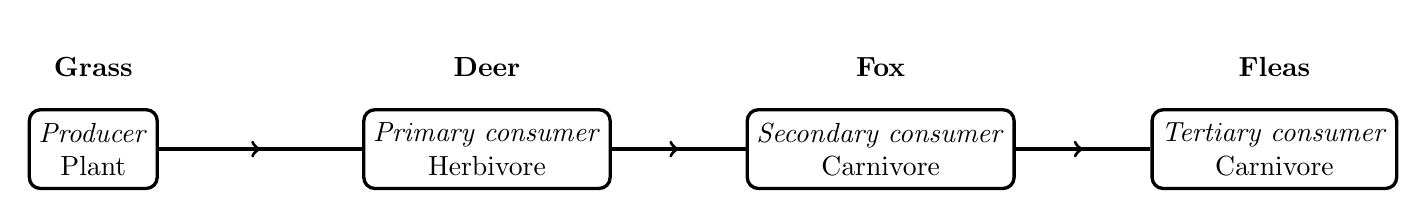
\begin{tikzpicture}[ 
		node distance=5cm, 
		very thick, 
		decoration={
			markings,
			mark=at position 0.5 with {\arrow{>}}
		},
		rounded corners,
		minimum size=1cm,
		every text node part/.style={align=center}
    ] 
	\node[draw, label=above:\textbf{Grass}] (prod) {\emph{Producer} \\ Plant};
	\node[draw, right of=prod, label=above:\textbf{Deer}] (primCons) {\emph{Primary consumer} \\ Herbivore};
	\node[draw, right of=primCons, label=above:\textbf{Fox}] (secCons) {\emph{Secondary consumer} \\ Carnivore};
	\node[draw, right of=secCons, label=above:\textbf{Fleas}] (tertCons) {\emph{Tertiary consumer} \\ Carnivore};

	\draw[postaction={decorate}] (prod) -- (primCons);
	\draw[postaction={decorate}] (primCons) -- (secCons);
	\draw[postaction={decorate}] (secCons) -- (tertCons);
\end{tikzpicture}

\vspace{3cm}
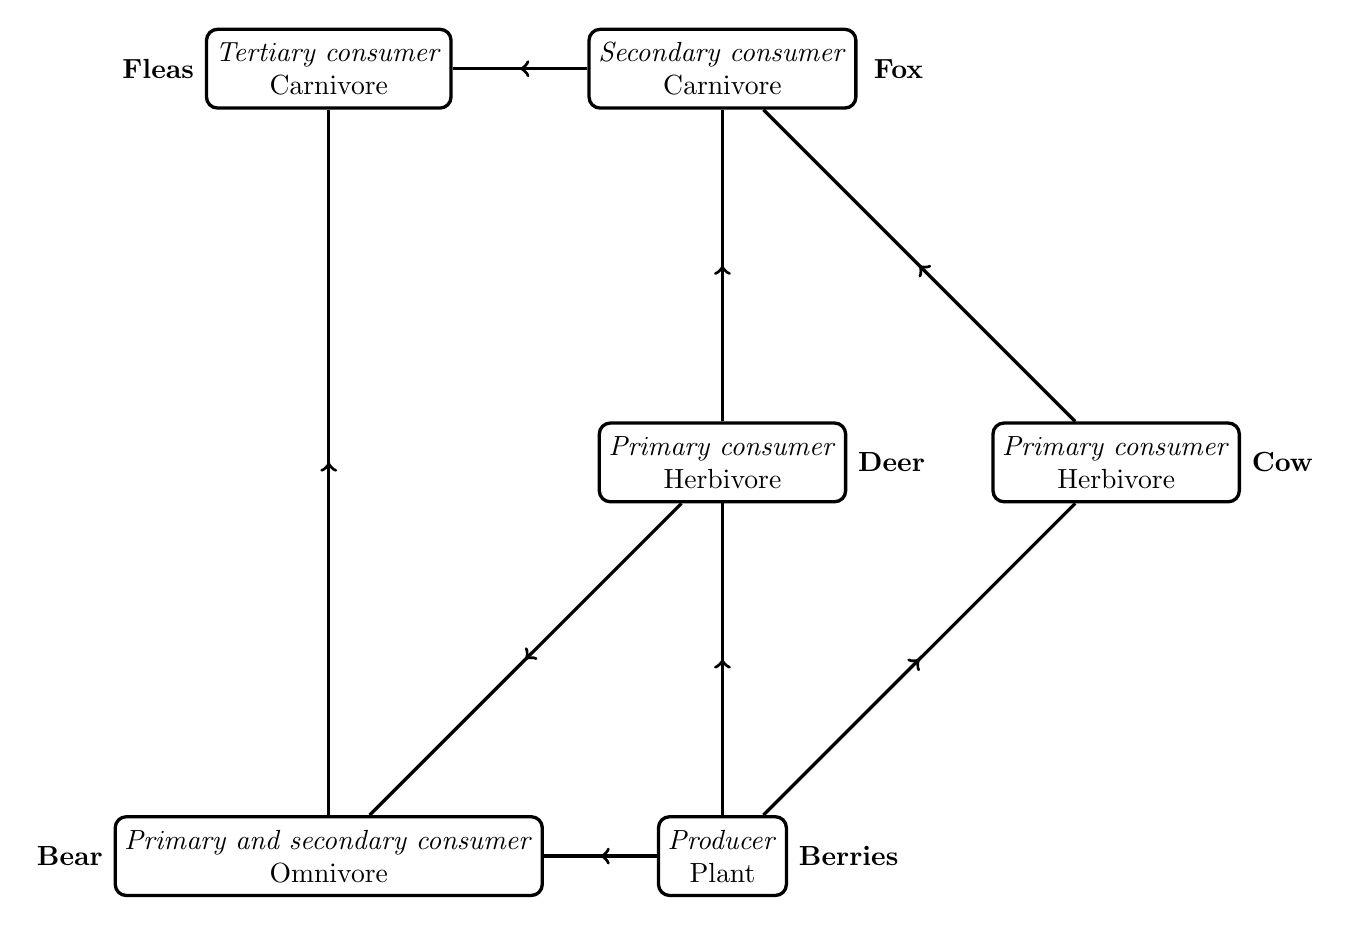
\begin{tikzpicture}[ 
		node distance=5cm, 
		very thick, 
		decoration={
			markings,
			mark=at position 0.5 with {\arrow{>}}
		},
		rounded corners,
		minimum size=1cm,
		every text node part/.style={align=center}
    ] 

	\node[draw, label=right:\textbf{Berries}] (prod) {\emph{Producer} \\ Plant};
	\node[draw, label=right:\textbf{Deer}, above of=prod] (deer) {\emph{Primary consumer} \\ Herbivore};
	\node[draw, label=right:\textbf{Cow}, right of=deer] (cow) {\emph{Primary consumer} \\ Herbivore};
	\node[draw, label=right:\textbf{Fox}, above of=deer] (fox) {\emph{Secondary consumer} \\ Carnivore};
	\node[draw, label=left:\textbf{Bear}, left of=prod] (bear) {\emph{Primary and secondary consumer} \\ Omnivore};
	\node[draw, label=left:\textbf{Fleas}, left of=fox] (fleas) {\emph{Tertiary consumer} \\ Carnivore};

	\draw[postaction={decorate}] (prod) -- (bear);
	\draw[postaction={decorate}] (prod) -- (deer);
	\draw[postaction={decorate}] (prod) -- (cow);
	\draw[postaction={decorate}] (cow) -- (fox);
	\draw[postaction={decorate}] (deer) -- (fox);
	\draw[postaction={decorate}] (deer) -- (bear);
	\draw[postaction={decorate}] (fox) -- (fleas);
	\draw[postaction={decorate}] (bear) -- (fleas);
\end{tikzpicture}

\vspace{3cm}
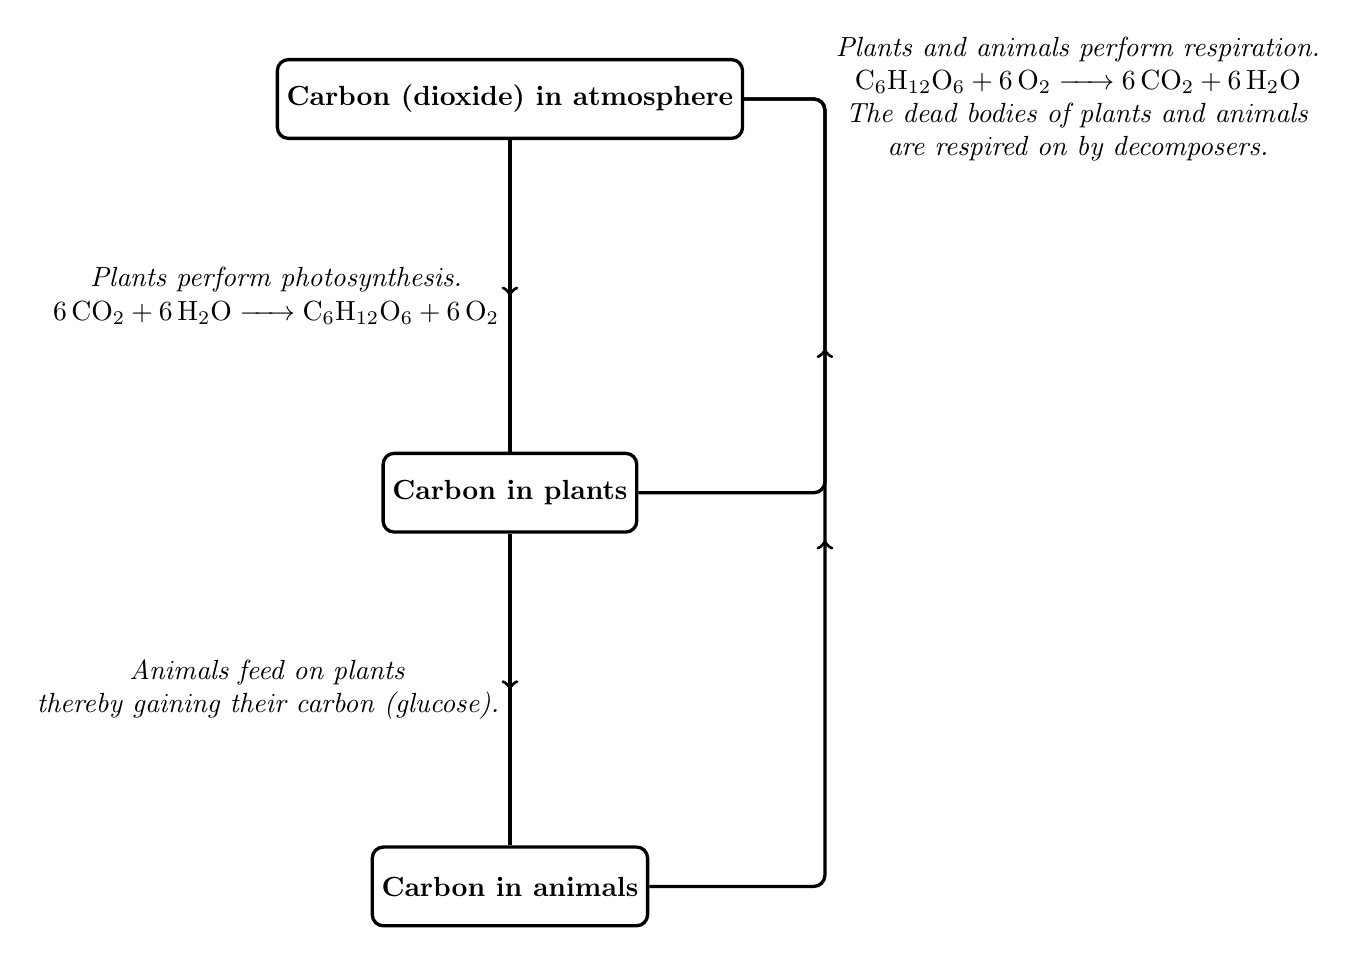
\begin{tikzpicture}[ 
		node distance=5cm, 
		very thick, 
		decoration={
			markings,
			mark=at position 0.5 with {\arrow{>}}
		},
		rounded corners,
		minimum size=1cm,
		every text node part/.style={align=center}
    ] 

	\node[draw] (atmos) {\textbf{Carbon (dioxide) in atmosphere}};
	\node[draw, below of=atmos] (plants) {\textbf{Carbon in plants}};
	\node[draw, below of=plants] (animals) {\textbf{Carbon in animals}};

	\draw[postaction={decorate}] (atmos) -- (plants) 
		node[left, midway]{\textit{Plants perform photosynthesis.} \\ \ce{6CO2 + 6H2O -> C6H12O6 + 6O2}};
	\draw[postaction={decorate}] (plants) -- (animals) 
		node[left, midway]{\textit{Animals feed on plants} \\ \textit{thereby gaining their carbon (glucose).}};
\draw [postaction={decorate}] (plants) -- ++ (4cm,0) |- node[anchor=west, midway]{\textit{Plants and animals perform respiration.} \\ \ce{C6H12O6 + 6O2 -> 6CO2 + 6H2O} \\ \textit{The dead bodies of plants and animals} \\ \textit{are respired on by decomposers.}} (atmos);
	\draw [postaction={decorate}] (animals) -- ++ (4cm,0) |- (atmos);
\end{tikzpicture}

\end{document}
